\section[2]{Existing Adaptive SPS}
\begin{frame}{Existing Adaptive SPS}
	Adaptive SPS can modify the number of replicas
	
	\begin{figure}
		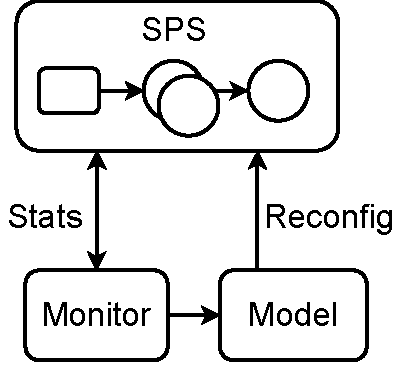
\includegraphics[scale=0.5]{images/concepts/RW-Automatic.pdf}
	\end{figure}
	
	There are two approaches:
	\begin{itemize}
		\item Reactive approach
		\item Predictive approach
	\end{itemize}
\end{frame}

\begin{frame}{Reactive approach}
	\begin{itemize}
		\item Statistics via a monitor
		\item Operator state analysis using thresholds
	\end{itemize}
	
	\begin{figure}
		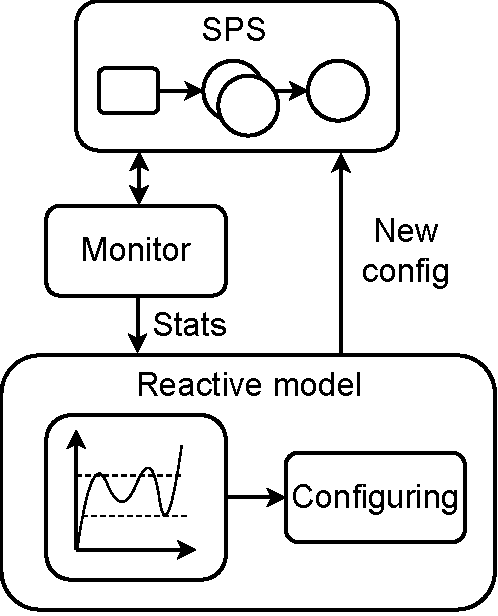
\includegraphics[scale=0.45]{images/concepts/RW-Reactive.pdf}
	\end{figure}
\end{frame}

\begin{frame}{Reactive approach}
	Metrics:
	
	\begin{itemize}
		\item CPU [\cite{GulisanoJPSV12}]
		\item Latency [\cite{MadsenZS16, SatzgerHLD11, HeinzeJHF14}]
		\item Throughput [\cite{KahveciG20, RussoCCP21, GedikSHW14}]
	\end{itemize}
	
	\pause
	
	\begin{alertblock}{Limitation}
		Most solutions consider a single metric
	\end{alertblock}
\end{frame}

\begin{frame}{Predictive approach}
	\begin{itemize}
		\item Based on prediction to determine the SPS reconfiguration
		\item Apply a predictor model
	\end{itemize}
	
	\begin{figure}
		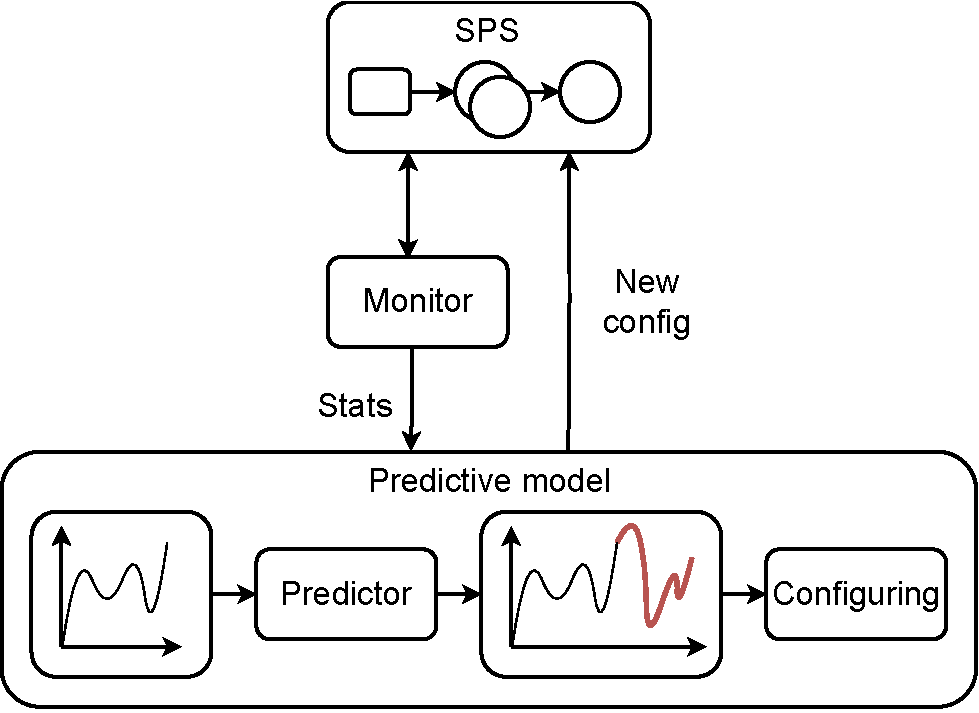
\includegraphics[scale=0.45]{images/concepts/RW-Predictive.pdf}
	\end{figure}
\end{frame}

\begin{frame}{Related Work}
	Predictor models:
	
	\begin{itemize}
		\item Reinforcement learning [\cite{CardelliniPNR18}]
		\item Time series [\cite{KombiLLRB19}]
		\item Fuzzy logic [\cite{MencagliTD18}]
		\item ANN [\cite{LombardiABQ18}]
	\end{itemize}
	
	\pause
	
	\begin{alertblock}{Limitation}
		Predictive models are specific to an input rate or scenario
	\end{alertblock}
\end{frame}





